\documentclass[withoutpreface,bwprint]{../cumcmthesis} %去掉封面与编号页
\usepackage{verbatim}
\usepackage{url}
\usepackage{pdfpages}
\usepackage{graphicx}
\usepackage{listings}
\usepackage{subcaption}%插入子图
% \usepackage{subfig}
\usepackage{float}
\usepackage{longtable,tabularx}
\usepackage{ltablex}
\keepXColumns
\usepackage{threeparttable}
\usepackage{cite,bookmark}
\title{latex使用指南}
\newcommand{\cnabstractname}{摘要}
\newenvironment{cnabstract}{%
  \par\small
%   \noindent\mbox{}\hfill{\bfseries \cnabstractname}\hfill\mbox{}\par
  \vskip 2.5ex}{\par\vskip 2.5ex}
\newcolumntype{Y}{>{\centering\arraybackslash}X}

\begin{document}
\maketitle
\begin{cnabstract}
  \textbf{摘要: }
  对latex中高频使用的语法进行记录
  \par\textbf{关键字: } %网络爬虫\quad 多元线性回归模型\quad 回归模型的检验
  %“\par在段首,表示另起一行,“\textbf{}”,花括号内的内容加粗显示
\end{cnabstract}
\tableofcontents
\newpage
\section{文档结构组织}
\subsection{input vs. include}
文档结构组织主要是在应对需要编译的latex文档过长时需要面临的问题,这里结合文档较长时存在的问题来分析\verb|\input|和\verb|\include|命令:
\begin{itemize}
  \item 文档较长时,tex代码较长,文本编辑器的功能会大打折扣。这时很自然地想要将文档拆分成多个tex文件,在编译时同时引入,这时就可以使用\verb|\input{文件名}|命令,扩展名(.tex)可省略,\textbf{支持嵌套}
  \item 文档较长,当进行细微调整时编译时间较长,这时可以考虑结合使用\verb|\includeonly{文件列表}|\\和 \verb|\include{文件名}|命令\footnote{includeonly是导言区命令,如单独使用include,相当于input命令,不过会在插入tex代码前后都有换页符},这么做的好处是能提高速度——对于只存在于文件列表内的文件,latex只会加载其对应的章节标题等信息,并不会将文档内容引入,这能保证对单个文档进行修改时仍能保持和整体文档一致的效果,大大提高了编译速度,不过需要注意的是\verb|\include{}|命令\textbf{不可以嵌套使用}
\end{itemize}
\subsection{插入pdf}
latex插入pdf时的两种常用方法及其优缺点表述如下:
\begin{itemize}
  \item $graphicx$是对$graphics$宏包的扩展或者增强,两个宏包的参数格式有细微差别,后者更多是对前者的补充。因为可以将pdf使用\verb|\includegraphics|引入,所以可以将其放置在浮动体或者直接插入到文档中,其相当于将pdf当做源文件的一部分插入在文档中,对其进行修改或者加以说明都会更方便一些,就个人体验而言更实用一些。
  \item $pdfpages$提供了很多选项来插入PDF文件,其在文档中写到避免产生类似$graphicx$插入pdf‘Overfull \verb|\hbox|’ and ‘Overfull \verb|\vbox|’ warnings的提示。自己在使用过程中的体验是该宏包适合用来pdf作为一个\textbf{独立的页面}插入到源文档中的情况,提供了丰富的命令对插入pdf的大小和原页面的大小进行调整,但是如果想对插入的pdf进行局部的调整或者加一个标题之类的操作,相对来说明比较麻烦且排版效果也比较差。
\end{itemize}
如想将导入的pdf双栏排列,建议使用$graphicx$宏包,双栏排列方法见小节:\nameref{双栏}
% \includepdf{../asset/cover.pdf}
\section{浮动体环境}
一般来说,为了排版的美观,都会将表格图片等内容放入浮动体环境,这块主要是针对插入的图片或者表格过大的情况作说明。
\subsection{插入图片}
图片过大的问题相对容易解决,只需要直接在修改\verb|width|的可选参数即可,引用图片\ref{sum_production}
\begin{figure}[H]%H定义浮动体位置,Here
  \small
  \centering
  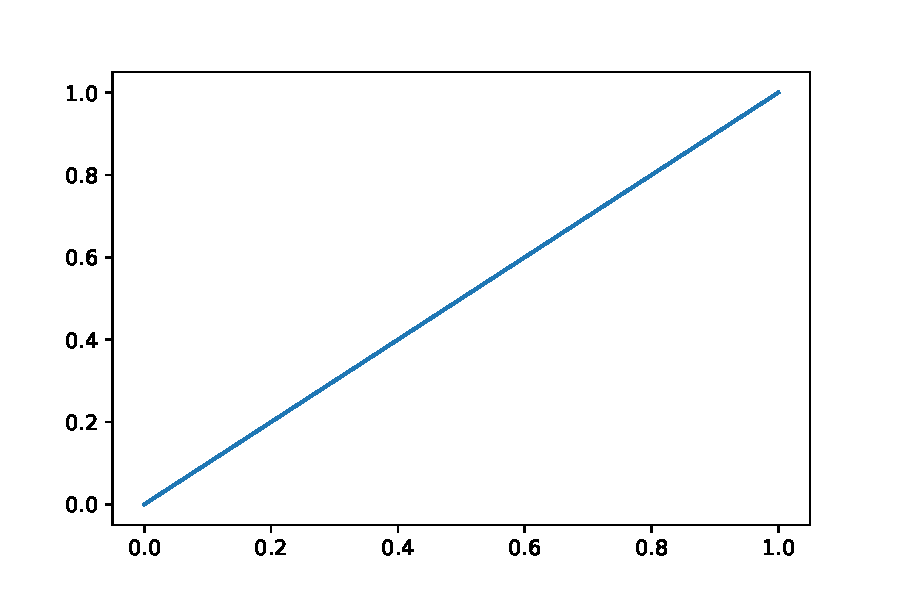
\includegraphics[width=\textwidth]{./asset/figure.pdf}
  \caption{全国煤炭企业前50强产煤总量}\label{sum_production}
\end{figure}
\subsubsection{图片/pdf并列排版}\label{双栏}
在引入pdf或者图片时(insert graphics),为节省页面空间,很多时候将两张图片进行双栏并排显示是一种不错的选择,这也就使用到了浮动体的双栏,这里给出一种比较简单的浮动体双栏排列的方法:
\lstinputlisting[language=tex]{./tex代码/picture_typest/two_pics_parral_subcaption.tex}
排版效果见图 \ref{sub_cap},
{
  % \usepackage{subcaption}浮动体双栏显示
\begin{figure}[H]
    \centering
    \begin{subfigure}{0.45\textwidth}
        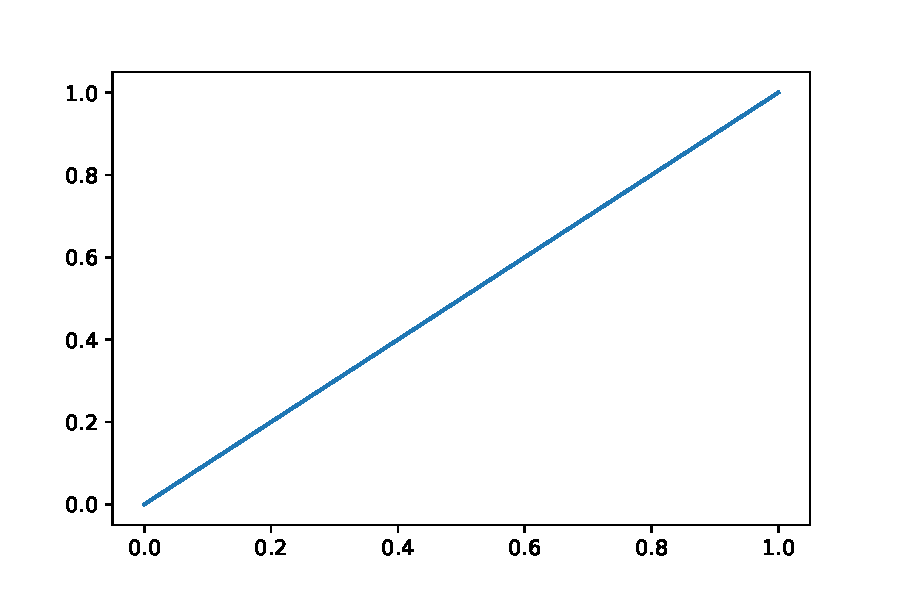
\includegraphics[width=\textwidth]{./asset/figure.pdf}
        \caption{题注1}
    \end{subfigure}
    \begin{subfigure}{0.45\textwidth}
        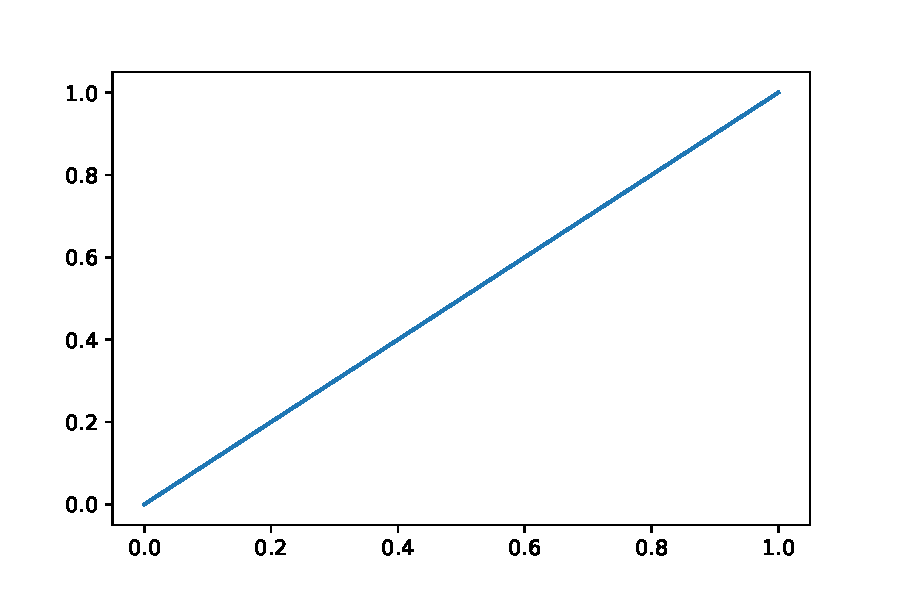
\includegraphics[width=\textwidth]{./asset/figure.pdf}
        \caption{题注2}
    \end{subfigure}
    \caption{两个图并排放置}\label{sub_cap}
  \end{figure}
}

除此以外还有一种解决方案是使用\verb|subfigure|,二者的区别可能主要在于三四个子图排列的便捷性上,我不使用这个功能所以也没细致研究,这里给出一个\verb|subfigure|的例子,貌似二者会有冲突,随便用哪种方法好了。
\lstinputlisting[language=tex]{./tex代码/picture_typest/two_pics_subfig.tex}
% 排版效果见图 %\ref{sub_fig},
% {%\usepackage{subfig}
\begin{figure}[H]
    \centering
    \subfloat[传统交叉验证]{
        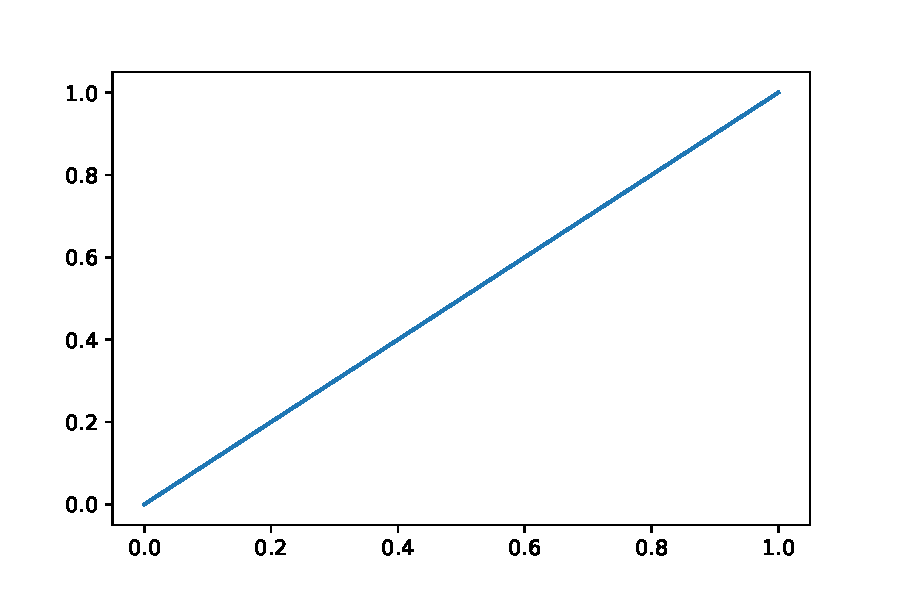
\includegraphics[width=0.48\textwidth]{./asset/figure.pdf}
        \label{fig:cv-传统}}
    \subfloat[时间序列的交叉验证]{
        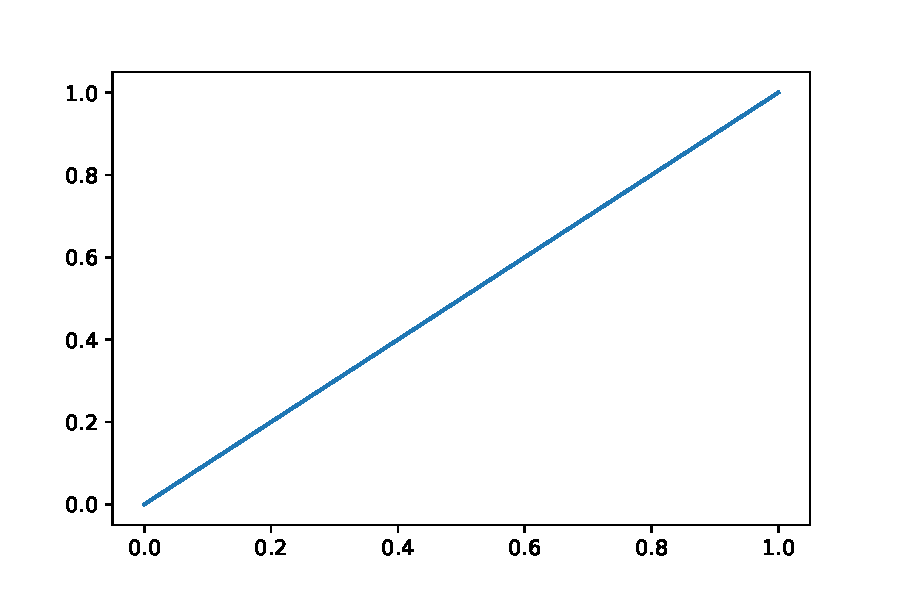
\includegraphics[width=0.48\textwidth]{./asset/figure.pdf}
        \label{fig:cv-时序}}
    \caption{两种交叉验证方式的对比(以五折交叉验证为例)}\label{sub_fig}
  \end{figure}
% }
\subsection{插入表格}
一般来插入的表格都可以通过python的\verb|DataFrame.to_latex()|函数来导出到指定位置,然后通过\verb|input|命令导入使用,经常会用到的导出模板为:
\begin{lstlisting}[language=python]
df.to_latex('./排版/tex代码/cr8.tex',caption='($CR_8$)计算结果',label='table',header=False)
\end{lstlisting}
只需微调函数的参数即可,注意如下:
\begin{itemize}
  \item 列名如果有数学公式的话导出会加转义符,这样在latex编译后不能正常显示。可以设置\verb|escape=False|解决这个问题,不过这样设置数值中的转义符号也会被取消掉,这点在对于数值列中含有"\%"的数据中需要注意
  \item 不想显示index列或者列名列可以通过调节\verb|index|和\verb|header|参数进行修改
  \item 修改表格中数字位数可以通过\verb|float_format|参数进行修改,一个例子是"\%.2f"。
\end{itemize}

插入表格的情况,相对复杂,可能出现的问题包括引入的表格过宽和过长的问题。
一个简单的例子如表\ref{tab:table1}:
{\begin{table}[h]
\centering
\caption{A simple Table}
\label{tab:table1}
\begin{tabular}{rl}
\toprule
 A & B \\
\midrule
 1 & a \\
 2 & b \\
 3 & c \\
 4 & d \\
\bottomrule
\end{tabular}
\end{table}
}
\subsubsection{宽表的缩窄(tabular)}
针对插入表格\textbf{过宽}的情况
\begin{enumerate}
  \item 一般选择使用\verb|graphicx|宏包提供的\verb|\resizebox{h-length%l}{v-length%l}{text}|命令来解决。这里给一个示例,语法如表\ref{cr8table}所示(代码在\verb|tex代码|文件夹的\verb|widetable|里边。
        {
        \begin{table}[H]
    \centering
    \caption{近十年行业集中率($CR_8$)计算结果}
    \label{cr8table}
    \resizebox{\linewidth}{!}{
        \begin{tabular}{llllllllllll}
            \toprule
            年份               & 2011     & 2012     & 2013     & 2014     & 2015     & 2016     & 2017     & 2018    & 2019     & 2020     & 2021    \\
            行业集中率($CR_8$) & 0.288718 & 0.301209 & 0.316948 & 0.331046 & 0.360429 & 0.359104 & 0.346434 & 0.40707 & 0.404583 & 0.477353 & 0.49315 \\
            \bottomrule
        \end{tabular}
    }
\end{table}

        }
  \item 除了缩小表格内容以外,对于宽度溢出不太严重的表格,也可以选择修改水平排版开始位置,这也能使得本来溢出的表格可以被放下,而且也不会导致字体看起来太小(示例如表\ref{cr8.1}所示)
        {
        \begin{table}[H]
    \centering
    \caption{近十年行业集中率($CR_8$)计算结果}
    \label{cr8.1}
    \setlength{\leftskip}{-60pt}
    \begin{tabular}{lllllllll}
        \toprule
        年份               & 2011     & 2012     & 2013     & 2014     & 2015     & 2016     & 2017     & 2018                \\
        行业集中率($CR_8$) & 0.288718 & 0.301209 & 0.316948 & 0.331046 & 0.360429 & 0.359104 & 0.346434 & 0.40707    \\
        \bottomrule
    \end{tabular}
\end{table}

        }
\end{enumerate}

\subsubsection{窄表的定宽处理(tabularx)}
刘海洋老师的书里有写到,可以去翻翻。用的是\verb|tabularx|环境,自己定义了一种新的列格式\footnote{自适应调整列,默认向左对齐,可以自己定义一个居中的列形式,具体见表源码}(X),因为是起于\verb|tabular|所以相对来说比较好用。效果大概是下边这样:
% \newcolumntype{Y}{>{\centering\arraybackslash}X} 居中列的定义
\begin{table}[H]
    \caption{序列平稳性检验结果(ADF)}
    \label{adf-test}
    \begin{tabularx}{\textwidth}{YY}
    \toprule
    指标 & 取值 \\
    \midrule
    检验统计量 & -11.65 \\
    p值 & 0.00 \\
    滞后阶数 & 22.00 \\
    样本数量 & 3660.00 \\
    % Critical Value (1\%) & -3.43 \\
    % Critical Value (5\%) & -2.86 \\
    % Critical Value (10\%) & -2.57 \\
    \bottomrule
    \end{tabularx}
    \end{table}
    

这种环境不能使用Python的\verb|to_latex|直接导出,

\subsubsection{长表格}
\textbf{python函数原生支持的方法,主要问题是如果是一个窄表调成定宽比较麻烦}:
长表格主要使用的是\verb|longtable|宏包的longtable环境(使用说明可以看刘海洋的教程),与tabular类似,不过多了一些处理跨页操作的命令。因为\verb|to_latex|函数可以直接导出这种样式的表格,所以在实际中使用这种表格的频率也比较高,想要导出这种环境的表格时,只需在开始提到的模板中加入\verb|longtable=True|的参数即可获得,使用比较方便\footnote{longtable的表格宽度是根据表格内容调整的,当表格属于长而窄的类型时美观度比较有限,这时可以考虑利用python的concat函数对长表格进行拆分和列拼接}。\par
\textbf{注意}:长表格不支持\verb|resizebox{h-length}{v-length}{text}|命令来自适应调节表格的宽度,遇到表格宽度过大的情况,推荐适当缩小表格字体( 在表格外添加 \verb|\footnotesize|  命令 ) 或者对表格的结构进行调整,具体效果如表 \ref{num_var_desc}所示。\par

{
  % \tabcolsep=0.00cm
% \resizebox{1.0\linewidth}{!}{
  \footnotesize{\small}
  \begin{longtable}{lccccccc}
  % \begin{tabularx}{\linewidth}{lccccccc}
  \caption{数值变量描述统计结果} \label{num_var_desc} \\
  \toprule
  特征 & 最小值 & 25\%分位 & 中位数 & 75\%分位 & 最大值 & 均值 & 标准差 \\
  \midrule
  \endfirsthead
  \caption[]{数值变量描述统计结果} \\
  \toprule
  特征& 最小值 & 25\%分位 & 中位数 & 75\%分位 & 最大值 & 均值 & 标准差 \\
  \midrule
  \endhead
  \midrule
  \multicolumn{8}{r}{见下页} \\
  \midrule
  \endfoot
  \bottomrule
  \endlastfoot
  流失标志(Attrition\_Flag) & 0.00 & 0.00 & 0.00 & 0.00 & 1.00 & 0.16 & 0.37 \\
  年龄(Customer\_Age) & 26.00 & 41.00 & 46.00 & 52.00 & 73.00 & 46.33 & 8.02 \\
  家属人数(Dependent\_count) & 0.00 & 1.00 & 2.00 & 3.00 & 5.00 & 2.35 & 1.30 \\
  开户时长(Months\_on\_book) & 13.00 & 31.00 & 36.00 & 40.00 & 56.00 & 35.93 & 7.99 \\
  产品总数(Total\_Relationship\_Count) & 1.00 & 3.00 & 4.00 & 5.00 & 6.00 & 3.81 & 1.55 \\
  {过去一年不活跃月数(Months\_Inactive\_12\_mon)} & 0.00 & 2.00 & 2.00 & 3.00 & 6.00 & 2.34 & 1.01 \\
  {过去一年签订合约数(Contacts\_Count\_12\_mon)} & 0.00 & 2.00 & 2.00 & 3.00 & 6.00 & 2.46 & 1.11 \\
  卡限额(Credit\_Limit) & 1438.30 & 2555.00 & 4549.00 & 11067.50 & 34516.00 & 8631.95 & 9088.78 \\
  卡待还余额(Total\_Revolving\_Bal) & 0.00 & 359.00 & 1276.00 & 1784.00 & 2517.00 & 1162.81 & 814.99 \\
  可用额度(Avg\_Open\_To\_Buy) & 3.00 & 1324.50 & 3474.00 & 9859.00 & 34516.00 & 7469.14 & 9090.69 \\
  交易金额(Total\_Trans\_Amt) & 510.00 & 2155.50 & 3899.00 & 4741.00 & 18484.00 & 4404.09 & 3397.13 \\
  交易金额变动(Total\_Amt\_Chng\_Q4\_Q1) & 0.00 & 0.63 & 0.74 & 0.86 & 3.40 & 0.76 & 0.22 \\
  交易次数(Total\_Trans\_Ct) & 10.00 & 45.00 & 67.00 & 81.00 & 139.00 & 64.86 & 23.47 \\
  交易次数变动(Total\_Ct\_Chng\_Q4\_Q1) & 0.00 & 0.58 & 0.70 & 0.82 & 3.71 & 0.71 & 0.24 \\
  平均使用率(Avg\_Utilization\_Ratio) & 0.00 & 0.02 & 0.18 & 0.50 & 1.00 & 0.27 & 0.28 \\
  \end{longtable}
  % \end{tabularx}


% % 导言区使用 \usepackage{longtable}
% \newcommand\meta[1]{\emph{$\langle$#1$\rangle$}}
% \begin{longtable}{|l|l|}
% \caption{\texttt{longtable} 环境中的命令汇总} \\
% \hline
% \endfirsthead
% \multicolumn{2}{l}{(续表)} \\
% \hline
% \endhead
% \hline
% \multicolumn{2}{c}{\itshape 接下一页表格……} \\[2ex]
% \endfoot
% \hline
% \endlastfoot
% \multicolumn{2}{|c|}{环境的水平对齐可选项} \\ \hline
% 留空 & 表格居中%
% \footnote{实际上,留空的对齐方式是由一组命令控制的,参见宏包文档。} \\
% \verb=[c]= & 表格居中 \\
% \verb=[l]= & 表格左对齐 \\
% \verb=[r]= & 表格右对齐 \\
% \hline \multicolumn{2}{|c|}{结束表格一行的命令} \\ \hline
% \verb=\\= & 普通的结束一行表格 \\
% \verb=\\[=\meta{距离}\verb=]= & 结束一行,并增加额外间距 \\
% \verb=\\*= & 结束一行,禁止在此分页 \\
% \verb=\kill= & 当前行不输出,只参与宽度计算 \\
% \verb=\endhead= & 此命令以上部分是每页的表头 \\
% \verb=\endfirsthead= & 此命令以上部分是表格第一页的表头 \\
% \verb=\endfoot= & 此命令以上部分是每页的表尾 \\
% \verb=\endlastfoot= & 此命令以上部分是表格最后一页的表尾 \\
% \hline \multicolumn{2}{|c|}{标题命令} \\ \hline
% \verb=\caption{=\meta{标题}\verb=}= & 生成带编号的表格标题 \\
% \verb=\caption*{=\meta{标题}\verb=}= & 生成不带编号的表格标题 \\
% \hline \multicolumn{2}{|c|}{分页控制} \\ \hline
% \verb=\newpage= & 强制分页 \\
% \verb=\pagebreak[=\meta{程度}\verb=]= & 允许分页的程度(0--4) \\
% \verb=\nopagebreak[=\meta{程度}\verb=]= & 禁止分页的程度(0--4) \\
% \hline \multicolumn{2}{|c|}{脚注控制} \\ \hline
% \verb=\footnote= & 使用脚注\footnote{普通表格中不能用。},
%   注意不能用在表格头尾 \\
% \verb=\footnotemark= & 单独产生脚注编号,不能用在表格头尾 \\
% \verb=\footnotetext= & 单独产生脚注文字 \\
% \hline \multicolumn{2}{|c|}{长度参数} \\ \hline
% \verb=\LTleft= & 对齐方式留空时,表格左边的间距,默认为 \verb=\fill= \\
% \verb=\LTright= & 对齐方式留空时,表格右边的间距,默认为 \verb=\fill= \\
% \verb=\LTpre= & 表格上方间距,默认为 \verb=\bigskipamount= \\
% \verb=\LTpost= & 表格下方间距,默认为 \verb=\bigskipamount= \\
% \verb=\LTcapwidth= & 表格标题的宽度,默认为 4\,in \\
% \end{longtable}

}

\textbf{长窄表调成定宽}:这时无法沿用resizebox的思路,主要是因为longtable环境和tabular环境不兼容,一个新的解决方案是使用\verb|ltablex|宏包,这个宏包是对\verb|longtable|和\verb|tabularx|的结合,可以实现长表格的定宽,它使用longtable环境定义长表的语法同时支持tabularx环境的列格式定义,具体可以看long\_table.tex文件,记得在导言区添加\verb|\usepackage{ltablex}|命令和\verb|\keepXColumns|命令。

\section{插入题注}
这是一个题注\footnote{使用比较简单,这里不再赘述}。
\section{导入参考文献}
参考文献的导入主要是使用zotero先导出bib文件。引文格式可能需要根据不同的使用场景进行调整。
\subsection{biblatex宏包}
\verb|biblatex|宏包提供了比较全面的中文参考文献导入支持,需要注意的是在编译bib文件时默认使用\verb|biber|后端,同时在生成和导入参考文献时与其它宏包有所区别:
\begin{verbatim}
\documentclass{ctexart}
% 使用符合 GB/T 7714-2015 规范的参考文献样式
\usepackage[style=gb7714-201,backend=bibtex]{biblatex}
% 注意加 .bib 扩展名
\addbibresource{egbibdata.bib}
\begin{document}
见文献\cite{caimin2006}。
\printbibliography%插入参考文献
\end{document}
\end{verbatim}\par
\subsection{中文文献的自定义导入}
对于中文文献,可以使用\verb|gbt7714|宏包来生成满足我国标准的参考文献格式:
\begin{verbatim}
\documentclass{ctexart}
\usepackage{gbt7714}
\bibliographystyle{gbt7714-numerical}
\begin{document}
\cite{...}
...
\bibliography{bibfile}
\end{document}
\end{verbatim}\par
这种宏包导入有一个比较麻烦的是作者在参考文献中出现的位置问题,经测试该库不会自动按照bib文件中作者的顺序排列,在多位作者同时完成一篇文章时排序混乱,官方文档提供了一种解决方案,但是比较麻烦,推荐使用\verb|biblatex|宏包。\verb|gbt7714|宏包的好处是它对中文文献的引用格式和参考文献的样式有比较好的支持。

按照国标的规定,参考文献的标注体系分为“顺序编码制”和“著者-出版年制”。用户应在导言区调用宏包 gbt7714,并且使用 \verb|\bibliographystyle| 命令选择参考文献
表的样式,比如:
\begin{verbatim}
\bibliographystyle{gbt7714-numerical} %顺序编码制
或者
\bibliographystyle{gbt7714-author-year} %著者-出版年制
\end{verbatim}
此外还可以使用 2005 版的格式 gbt7714-2005-numerical 和 gbt7714-2005-author-year。
另外几点注意:
\begin{itemize}
  \item 可以通过\verb|\citestyle{⟨citation style⟩}|命令来改变引用位置的显示格式,可选参数为super, numbers, author-year,在顺序编码制下默认引用格式为上角标(sub).
  \item 同一位置引用多篇文献时,如果想要在引用位置自动对文献进行排序则需要将\verb|sort&compress|传递给宏包的可选参数
        \begin{verbatim}
    \usepackage[sort&compress]{gbt7714}
  \end{verbatim}
\end{itemize}
\textbf{注意该宏包不要和cite宏包一同引入,会起冲突}。\par

\LaTeX 中更为常用的一种导入参考文献的格式,其中\verb|unsrt|样式表示参考文献条目按照文章中出现顺序排列。
%参考文献
\begin{verbatim}
\bibliographystyle{unsrt}
\bibliography{ref}
\end{verbatim}
该方法下在引用位置处显示是类似"[4]"的形式。
\newpage
%附录
\begin{appendices}
  \section{插入代码}
  \begin{lstlisting}[language=r]
data<-read.csv('./data.csv')
names(data)
# model<-lm(log(单价)~.-所属区-朝向-小区,data)
shapiro.test(log(data$单价))
shapiro.test(data$单价)
model <- lm(log(单价) ~ ., data)
summary(model)
sel_model <- step(model)
summary(sel_model)
# 多重共线性
library(car)
library(lmtest)
resettest(sel_model, power = 2)
library(lmtest)
bgtest(sel_model)
bptest(model)
library("ivreg")
model <- ivreg(log(单价) ~ 容积率 + 总楼栋数 + 房龄 + 客厅数 + 卫生间数 + 总楼层+绿化率 + 小区参考均价 | 容积率 + 总楼栋数 + 房龄 + 客厅数 + 卫生间数 +  总楼层+绿化率 + 交易价值 + 居住品质, data = data)
summary(model)
\end{lstlisting}
  \subsection{input方法}
  更为简洁的一种导入方法
  \lstinputlisting[language=python]{./asset/test.py}
\end{appendices}
\end{document}